\chapter{Construção do Guia de Implantação do Processo}
\label{sec:construcaoguiaimplantacao}

Este capítulo é destinado a explanar como o Guia de Implantação foi criado. Abaixo como este capítulo está organizado:

\begin{itemize}
\item Na Seção \ref{sec:consideracoesiniciais} é apresentado as considerações iniciais para esse capítulo.
\item Na seção \ref{sec:estruturaguiaimplantacao} é apresentado o guia de implantação como visão geral e sua estrutura.
\item Na seção \ref{sec:oguiadeimplantacao} mostra aspectos da construção do software que será usado como guia de implantação.
\item Na seção \ref{sec:consideracoesfinaisguiaimplantacao} a consolidação dos resultados obtidos neste capítulo são mostrados.
\end{itemize}

\section{Considerações Iniciais}
\label{sec:consideracoesiniciais}

Como mencionado no capítulo anterior, um dos componentes do \textit{framework} FreeTest é o guia de implantação, que consiste em um guia para implantação que viabiliza a utilização do Método FreeTest de forma fácil, objetiva e de modo \textit{As-a-Service}.

A intenção primária do guia de implantação é guiar as Organizações na implantação do processo do Método Freetest. Além da ferramenta de processo e modelagem dos mesmos, o guia de implantação corrobora de forma fácil, prática e intuitiva a implantação inicial do processo, sugere ferramentas de apoio à implantação da prática especifica em questão e ainda aborda técnicas aplicáveis no contexto da literatura e de mercado para se atingir os objetivos das Práticas Especificas que forem implantadas.

O software criado para ser o guia de implantação aborda critérios iniciais para implantação do processo, contudo pela sua concepção, é possível que Organizações possam realizar a manutenção do guia e dos processos, podendo assim evoluir e/ou estender o processo da forma que desejarem e customizada à suas necessidades.

\section{Estrutura do Guia de Implantação}
\label{sec:estruturaguiaimplantacao}

O guia de implantação aborda conhecimentos empíricos dos autores, juntamente com conhecimento cientifico obtido nas revisões da literatura, embasamento teórico, além de boas práticas da engenharia de software e áreas afins. As contribuições de como implantar uma prática especifica seguem vinculadas a cada prática especifica respectiva, deste modo, Organizações que desejam implantar uma prática especifica qualquer conseguirá encontrar as informações relevantes e de auxilio à implantação da tal prática neste guia.

As informações de como implantar a prática especifica podem ser encontradas diretamente na seção da prática especifica, na \textit{wiki} deste trabalho \footnote{http://wiki.freetestframework.com}. Como pode ser visto na figura \ref{fig:fig51} a seção de como implantar a prática especifica está vinculada a parte informativa da mesma.

\begin{figure}[H]
\centering
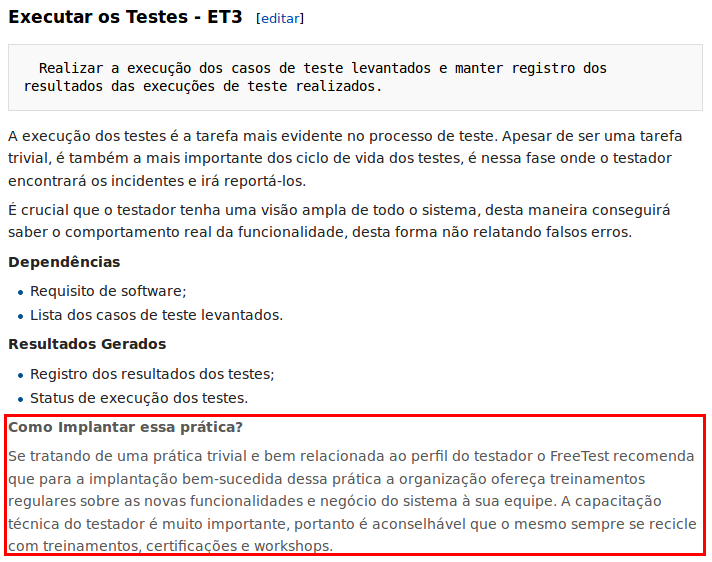
\includegraphics[width=.90\textwidth]{fig/figura51.png}
\caption{Estrutura do guia de implantação: "Como implantar essa prática?"}
\label{fig:fig51}
\end{figure}

A seguir nas próximas subseções podem ser vistos as instruções/sugestões de como implantar todas as práticas especificas sugeridas pelo FreeTest.

\subsection{Realizar análise de risco e definir estratégia de teste – GPT1}
\label{sec:guiagpt1}

Para realização de uma análise de riscos eficiente e definição de qual será a melhor estratégia de teste a ser utilizada é importante que a organização tenha uma documentação de testes mais completa possível. O Método FreeTest não indica um método ou ferramenta específica para levantamento e análise dos riscos, contudo orienta com algumas instruções que podem ser seguidas para que a organização consiga realizar uma análise de risco adequada aos projetos de teste. Uma das formas de se fazer uma análise de risco assertiva é respondendo as seguintes perguntas aos possíveis riscos \cite{Rios}:

\begin{itemize}
\item O risco é relevante para as atividades de teste?
\item Este risco está na alçada de responsabilidades da equipe de testes?
\item O risco é previsível porém não existe nenhuma certeza quanto a sua ocorrência futura?
\item O risco é significante para o projeto de testes?
\item O risco não está sendo tratado pelo plano de gerência de projeto de software?
\end{itemize}

Se a resposta para as perguntas acima foi um "Sim", os riscos devem ser registrados com as seguintes informações:

\begin{itemize}
\item Risco;
\item Tipo de Risco;
\item Probabilidade;
\item Impacto ou Criticidade;
\end{itemize}

\textbf{Sendo que:}

Risco, deve conter a uma descrição do risco em si. É importante que ela seja o mais detalhada possível, pois essa informação servirá como base para os futuros planos de teste.

Tipo de Risco, se tratando de riscos do produto, os riscos podem ser funcionais ou não funcionais neste último caso podem ser categorizados como: usabilidade, acessibilidade, segurança, performance, escalabilidade e segurança.

Probabilidade, é a chance de que o risco ocorra. A sugestão é que seja entre 10\% e 90\% e seja incrementado de 10 em 10. Sendo 0\% a probabilidade não precisa ser tratado, pois não terá chance de ocorrer e 100\% não será um risco e sim um problema já previsto.

Impacto ou Criticidade, a dica é que seja definida a criticidade com um ranking numa escala de 1 a 5, sendo:

\begin{itemize}
\item Impacto baixo no sucesso do projeto;
\item Impacto médio no sucesso do projeto;
\item Impacto alto no sucesso do projeto;
\item Impacto muito alto no sucesso do projeto;
\item Impacto que pode afetar seriamente o sucesso do projeto.
\end{itemize}

É importante que no planejamento dos riscos no ciclo de testes toda a equipe monitore os riscos com maior probabilidade e impacto. Para tanto, pode-se criar uma matriz de Probabilidade versus Impacto, multiplicando as probabilidades pelos Impactos, neste caso obtendo números entre 0,1 (10\% vezes 1) e 4,5 (90\% vezes 5). Pelo bom senso aconselha-se que a equipe monitore todos os riscos altos, ou seja, acima de 4.

Munido de todos os riscos mais relevantes, a equipe pode ter uma visão mais clara de quais riscos monitorar, caso tenha-se um número significante de riscos pode-se definir os TOP-10 maiores, utilizando a tabela mencionada anteriormente. Uma vez com os riscos definidos a equipe pode determinar qual a melhor estratégia tomar para a execução do projeto de teste.

A estratégia de teste por sua vez deverá ser cuidadosamente discutida, pois será peça chave para o sucesso do projeto. A estratégia de teste será fundamentada no escopo do projeto de testes e na análise de risco. Fazem parte da estratégia de teste os seguintes itens:

\begin{itemize}
\item Tipos de Teste que serão executados;
\item Automação dos testes e abordagens;
\item Testes de regressão ou não;
\item Técnicas de teste especifica para algum cenário peculiar.
\end{itemize}

Por fim, é muito importante que a equipe ou gestor mantenha todas essas informações bem documentadas. Outra prática recomendada é a criação de planos de contingência e mitigação dos riscos, utilizados sempre quando um risco se transformar em um problema e para reduzir a probabilidade de incidência do risco, respectivamente.

É importante que tais informações sejam sempre utilizadas como lições aprendidas e que sejam aproveitadas em outros projetos.

\subsection{Definir escopo de trabalho para o projeto – GPT2}
\label{sec:guiagpt2}

O FreeTest recomenda como implantação desta prática específica a criação da Estrutura Analítica do Projeto (EAP), como uma técnica para subdivisão das entregas e do trabalho do projeto em componentes menores e que permitirão o gerenciamento mais fácil.

Por definição uma EAP, segundo o PMBOK \cite{pmbok2014} é um recurso que tem como principal objetivo a divisão do projeto em partes menores (também chamadas de tarefas ou pacotes de trabalho). Consequentemente, estas partes se tornam mais fáceis de serem compreendidas pelos membros da equipe e gerenciadas pelo gestor do projeto.

O FreeTest recomenda as seguintes dicas para criação de uma EAP:

\begin{itemize}
	\item Decomponha a EAP em fases e atividades em níveis, que sejam fáceis de serem gerenciados;
	\item Planeje as entregas, não as ações. Neste caso serão os entregáveis do projeto, quando o mesmo é divido em entregas parciais ao seu cliente;
	\item Quebre os pacotes de trabalho em durações adequadas;
	\item Utilize modelos de EAP de projetos já finalizados. É importante a utilização da base histórica e das lições aprendidas em projetos anteriores.
\end{itemize}

\subsection{Estabelecer estimativas de tempo para realização de tarefas, criação de artefatos e preparação dos ambientes de trabalho – GPT3}
\label{sec:guiagpt3}

A escolha de qual método de estimativa utilizar está muito ligado ao perfil da organização. Normalmente a mesma técnica de estimativa é utilizada por toda a equipe, seja ela de desenvolvimento ou de teste. O FreeTest no entanto, indica algumas técnicas já consagradas, utilizados por equipes ágeis e tradicionais. Abaixo as técnicas recomendadas e como implantá-las na sua organização.

\textbf{\textit{Planning Poker}}\cite{Cohn2005} O \textit{Planning Poker} ou \textit{Scrum Poke}r tem o propósito de se obter a estimativa por meio de um jogo de cartas, deve permitir que todos os membros da equipe de forma heterogênea participem colocando a sua visão de complexidade, considerando o fator tempo e esforço para pontuar uma carta e após juntos chegar a um denominador comum na equipe através de consenso.

\textbf{Como Implantar o \textit{Planning Poke}r:}
\begin{itemize}
    \item O requisito/\textit{user story} é apresentado inicialmente a toda equipe. É interessante que o mesmo seja feito da forma mais clara e que o entendimento do mesmo seja geral. Neste momento a importância da aceitação do requisito é discutida (pelo \textit{Product Owner});
    \item Cada membro decide individualmente quantos \textit{Story Points} (valores abstratos que representam o tamanho, normalmente convertidos em horas) e seleciona a carta do seu baralho, sem mostrar aos demais;
    \item Quando todos os membros já estiverem com a carta escolhida em mãos, todos viram as cartas ao mesmo tempo;
    \item Caso haja uma discrepância muito grande nos valores, cada um apresenta uma justificativa. Normalmente quem tirou o valor mais alto ao mais baixo;
    \item Depois o time vota novamente até que o grupo chegue a um acordo.
\end{itemize}

\textbf{Estimativa de três pontos} – A estimativa de 3 pontos é uma técnica que permite refinar as estimativas considerando as incertezas e riscos. O conceito origina-se da Técnica de Revisão e Avaliação de Programa (PERT). Segundo o PMBOK \cite{pmbok2014}, “Uma técnica que usa três estimativas de custos ou duração para representar os cenários otimista, mais provável e pessimista. Esta técnica é aplicada para melhorar a exatidão das estimativas de custos ou duração quando não há certeza em relação à atividade subjacente ou ao componente de custo.”

\begin{itemize}
    \item Com os requisitos já levantados e divididos em pacotes de trabalho deve-se apresentá-los a toda a equipe;
    \item A equipe e/ou gerente de projetos solicita a estimativa para cada tarefa;
    \item O analista deverá definir o tempo otimista (o menor tempo para realizar a tarefa), provável (o tempo convencional) e o pessimista (o maior tempo possível para realizar a tarefa);
    \item Ao final encontra-se a média ponderada somando a estimativa pessimista, mais provável (multiplicado pela constante 4, certificando mais peso para essa variável) e otimista, em seguida o resultado é dividido por 6. O resultado dessa média será então a estimativa gerada pela técnica
\end{itemize}

É importante salientar que a escolha da técnica de estimativa está fortemente ligada à preferência da organização. O FreeTest recomenda as técnicas descriminadas acima, contudo não se opõe ao uso de outras técnicas e até mesmo incentiva a combinação entre técnicas diferentes.

\subsection{Planejar os recursos humanos - GPT4}
\label{sec:guiagpt4}

Uma boa maneira de planejar os recursos humanos ideais para as atividades específicas do projeto de teste é mantendo uma base de currículo de todos os integrantes da equipe. Tal prática apesar de trivial é pouco feita pelas organizações. O FreeTest ainda reforça que a gestão dessa base de currículo não seja simplesmente um arquivo com certificados e diplomas, mas sim um repositório com todas as informações mais atualizadas da equipe, contendo conhecimentos adquiridos durante os projetos, workshops ministrados e assistidos.

O FreeTest salienta também a importância de treinamentos recorrentes nas equipes. Em pequenas organizações onde o time é mais enxuto e heterogêneo é interessante que se faça com frequência workshops para disseminação de conhecimento. Essa prática além de promover o espírito colaborativo da equipe tornará o conhecimento tácito em explícito ajudando assim a gestão de conhecimento da organização.

\subsection{Determinar e documentar os riscos do projeto de teste, assim como seu impacto, probabilidade de ocorrência e prioridade de tratamento - GPT5}
\label{sec:guiagpt5}

Uma técnica simples que atende essa prática é a realização de \textit{brainstormings} com a intenção de obter uma lista completa dos riscos do projeto. O interessante é que toda a equipe participe, desta maneira uma equipe multidisciplinar tem mais chances de identificar, documentar, categorizar e criar planos de mitigação dos riscos.

É importante que todos os resultados encontrados durante as reuniões de \textit{brainstorming} sejam mantidos em uma base de dados, acompanhado de todas as informações inerentes ao risco, como impacto, probabilidade de ocorrência e planos de mitigação e resposta ao risco.

\subsection{Monitorar o progresso do projeto com relação ao estabelecido no planejamento e assessorar na realização de pendência - GPT6}
\label{sec:guiagpt6}

O monitoramento normalmente é feito por ferramentas de controle de projetos, no qual é possível avaliar o status e progresso das atividades. Uma técnica recomendada é a utilização de reuniões para acompanhamento do projeto com certa frequência, é possível, por exemplo manter uma rotina de reuniões diárias para que a equipe repasse o feedback das atividades e que ressalte qualquer problema ocorrido.

\subsection{Identificar casos de teste – ET1}
\label{sec:guiaet1}

Casos de teste podem ser identificados de diversas maneiras e descritos utilizando diversos métodos, desde descrições visuais como, mapas mentais à descrições textuais que são as mais comuns. A implantação dessa prática está ligada às preferências e tecnologias da organização, no entanto o FreeTest mostra algumas formas para identificação e documentação de casos de teste. As técnicas principais para a identificação e criação de casos de teste seguem abaixo:

\begin{itemize}
    \item \textbf{Particionamento por Classe de Equivalência} – O objetivo dessa técnica é eliminar os casos de testes redundantes dividindo as entradas de dados em classes de equivalência que serão testadas no lugar de toda a entrada. A criação de casos de teste para particionamento de equivalência é baseado numa avaliação das classes de equivalência para uma condição de entrada. ;
    \item \textbf{Análise de Valor Limite} - São casos de teste que exploram limites dos valores de entrada, neste caso tem mais probabilidade de encontrar defeitos. Os valores são escolhidos imediatamente acima ou abaixo dos limites definidos nas classes de equivalência.
\end{itemize}

Abaixo algumas dicas que podem ser seguidas para identificação de casos de teste, o FreeTest recomenda a utilização das técnicas já mencionada acima em combinação das instruções mostradas a seguir:

\begin{itemize}
    \item Utilize a documentação do software/negócio mais atualizada, caso não tenha documentação necessária, em linhas gerais defina o que deverá ser testado;
    \item Caso tenha documentação, como casos de uso, pode ser feito a derivação dos casos de teste a partir de sua estrutura padrão, utilizando basicamente dois métodos, derivação textual e visual
    \item \textbf{Derivação textual}: Sendo que para a derivação textual cada caminho deve ser mapeado, pois de cada caminho será extraído um requisito de teste.
    \item \textbf{Derivação visual}: Todo o caso de uso tem um desenho de todos os fluxos de eventos juntos, que pode ser usado como base na derivação visual;
    \item Se o sistema possui telas com muitos campos e com muitas probabilidades de situações, tais como regras de negócio, faça as combinações que você acha pertinentes em função das regras que seu teste pede. Neste caso é aconselhável usar teste por \textbf{tabela de decisões} se o nível de complexidade for alto ou médio;
    \item Use sempre técnicas como valor limite e particionamento por equivalência para reduzir e ser mais assertivo com seus casos de teste;
    \item Criar casos de teste para diversas situações em ambientes distintos, como banco de dados, resoluções de tela, plataformas e outros.
\end{itemize}

A criação de ambientes como mencionado anteriormente é inerente a forma de como a organização trabalha. No entanto, o FreeTest aconselha fortemente a criação de ambientes virtualizados, pois além de mais versáteis, menor custo é possível realizar o seu versionamento. Através do versionamento de ambientes é possível realizar \textit{rollbacks} do ambiente de forma mais ágil e flexível. Essa agilidade e flexibilidade na criação de ambientes torna as tarefas corriqueiras mais fáceis de serem realizadas, dessa forma fluindo melhor o processo e cumprindo melhor os prazos do projeto.

\subsection{Criar/atualizar ambiente de teste - ET2}
\label{sec:guiaet2}

A criação de ambientes como mencionado anteriormente é inerente a forma de como a organização trabalha. No entanto, o FreeTest aconselha fortemente a criação de ambientes virtualizados, pois além de mais versáteis, menor custo é possível realizar o seu versionamento. Através do versionamento de ambientes é possível realizar rollbacks do ambiente de forma mais ágil e flexível. Essa agilidade e flexibilidade na criação de ambientes torna as tarefas corriqueiras mais fáceis de serem realizadas, dessa forma fluindo melhor o processo e cumprindo melhor os prazos do projeto.


\subsection{Executar os Testes - ET3}
\label{sec:guiaet3}

Se tratando de uma prática trivial e bem relacionada ao perfil do testador o FreeTest recomenda que para a implantação bem-sucedida dessa prática a organização ofereça treinamentos regulares sobre as novas funcionalidades e negócio do sistema à sua equipe. A capacitação técnica do testador é muito importante, portanto é aconselhável que o mesmo sempre se recicle com treinamentos, certificações e workshops.

\subsection{Reportar e Acompanhar Incidentes - ET4}
\label{sec:guiaet4}

Não existe uma maneira “mais correta” de reportar um incidente, contudo seguem algumas informações importantes que se deve ter no relato de um incidente:

\begin{itemize}
    \item Prover aos desenvolvedores e outros envolvidos um retorno sobre o problema para permitir a identificação, isolamento e correção se necessário;
    \item Prover aos lideres de teste um meio para se rastrear a qualidade do sistema em teste e o progresso do teste;
    \item Prover ideias para aprimorar o processo de testes. Os detalhes de um relatório de incidente podem incluir: Data da emissão, autor, status e organização;
    \item Resultados esperados e resultados atuais;
    \item Identificação do item de teste (item de configuração) e ambiente;
    \item Processo do ciclo de vida do sistema ou software em que o incidente foi descoberto;
    \item Descrição do incidente para permitir a reprodução e resolução, incluindo \textit{logs}, \textit{database} \textit{dumbs}, ou \textit{screenshots};
    \item Escopo e grau de impacto para os \textit{stakeholder};
    \item Severidade do impacto no sistema;
    \item Urgência / Prioridade na correção;
    \item Estado (status) do incidente (aberto, rejeitado, duplicado, aguardando resolução, aguardando reteste ou fechado);
    \item Conclusão, recomendações e aprovações;
    \item Comentários gerais, tais como outras áreas que podem ser afetadas por uma mudança resultante de um incidente;
    \item Histórico de mudanças, como a sequência de ações tomadas pela equipe envolvida no projeto com respeito ao isolamento do incidente, reparo e confirmação da resolução;
    \item Referências, incluindo a identificação da especificação do caso de teste que revelou o problema;
    \item A estrutura de um relatório de incidente pode ser encontrada no "\textit{Standard for Software Test Documentation}" (IEEE Std. 829-1998) \cite{ieee829}.
\end{itemize}

\subsection{Encerrar teste - ET5}
\label{sec:guiaet5}

O FreeTest recomenda o uso de uma base de conhecimento para manutenção das informações importantes coletadas durante todo o ciclo de vida do projeto e ao término dele. Essas informações históricas, mantidas em um local apropriado guiará os próximos projetos a planejamentos mais assertivos e projetos menos suscetíveis a erros.

O uso de ferramentas para manutenção da base histórica é altamente recomendado. Pode-se ainda incluir relatos de acontecimentos peculiares ao projeto, informações sobre fatos que geraram algum transtorno e como resolvê-los, por exemplo, informações sobre dependências de bibliotecas de terceiros, configurações de ambientes e etc.

\subsection{Realizar verificação - RR1}
\label{sec:guiarr1}

O FreeTest recomenda que as revisões aconteçam de forma intercalada quando forem realizadas por profissionais que desempenham o papel de analista de requisitos e teste, e quando os papéis de analista requisito e teste forem feitos por pessoas diferentes a sugestão é que o testador que for fazer a revisão do requisito seja o mesmo que for testar o software. Desta maneira o testador estará munido de mais informações sobre os requisitos.

É Fundamental fazer um checklist com os principais erros e pontos relevantes. A criação de um checklist pode direcionar as revisões, tornando mais fácil e prático as sessões de revisão dos requisitos. A criação do checklist vai de acordo com as necessidades da organização, geralmente voltado para os erros mais comuns cometidos.

\subsection{Relatar e acompanhar inconsistências - RR2}
\label{sec:guiarr2}

O relato das inconsistências pode ser realizado utilizando uma ferramenta de bug tracker ou até mesmo inserindo comentários no texto revisado.

\subsection{Encerrar verificação - RR3}
\label{sec:guiarr3}

Aconselha o uso de uma ferramenta para o relato das inconsistências encontradas. As mesmas serão mantidas a título de base histórica para melhoramento continuo das atividades.

\subsection{Criar/Atualizar ambiente de teste - TDA1}
\label{sec:guiatda1}

A recomendação mais importante é que o ambiente de testes seja mais fiel ao ambiente de produção, pois assim, problemas relacionados com ambientes serão evidenciados durante os testes de aceite. O teste de aceitação é uma atividade muito importante para a entrega do software com qualidade e valor ao cliente, portante é importante que o mesmo seja feito de forma adequada e simulando aspectos e comportamentos que o ambiente do cliente proporciona.

\subsection{Executar teste de aceite - TDA2}
\label{sec:guiatda2}

O teste de aceitação tem como objetivo confirmar se o sistema está funcionando conforme o esperado, ou seja, prover a confiabilidade de que esteja de acordo com o requisito. Outro objetivo é avaliar se a qualidade do software, para prover informações sobre os riscos da implantação do sistema em um determinado momento aos gestores. Enfim, o objetivo principal do teste de aceitação não é encontrar defeitos e sim garantir a entrega de valor para o cliente.

\subsection{Encerrar teste de aceite - TDA3}
\label{sec:guiatda3}

Aconselha o uso de uma ferramenta para o relato das inconsistências encontradas. As mesmas serão mantidas a título de base histórica para melhoramento continuo das atividades.

% Identificar produtos de trabalho, tipos e critérios de revisão
% O ideal é que a organização realize a análise estática de código e revisão em pares de todo o código fonte possível. O critério de escolha para realização das revisões está muito relacionado ao perfil da equipe e efetivo de pessoas.
% A revisão em pares por ser uma prática mais “cara” pode ser reduzida a partes específicas do código, geralmente partes mais críticas e que contem mais lógicas de negócio. Outra maneira efetiva de escolher o que revisar é indicando analistas seniores para realizar o levantamento das áreas críticas do sistema, geralmente onde há muita dependência entre códigos fontes e/ou há muita regra de negócio.
% O FreeTest recomenda o uso de checklists de “boas práticas” contendo os critérios de revisão para orientar as sessões de revisão. Esse checklist é importante, pois guiará mais facilmente as revisões, principalmente quando o revisor não conhece bem os critérios usados para a revisão de código da organização.

\subsection{Identificar produtos de trabalho, tipos e critérios de revisão - AES1}
\label{sec:guiaaes1}

O FreeTest recomenda que o código escrito por um desenvolvedor, antes de ser enviado para o ambiente de produção, seja revisado por outro membro da equipe. Essas revisões podem ser feitas de diversas maneiras, como, por exemplo, programação em pares, ou mesmo realizando uma leitura/revisão sistemática do código. Após a revisão o revisor destaca todos as inconsistências encontrados e envia ao autor original do código. O autor do código avalia os comentários recebidos e eventualmente realiza as correções no código-fonte.
Uma boa dica para realizar a revisão é que desenvolvedores mais seniores o façam, pois como conhecem mais o software e regras de negócio poderão facilmente encontrar inconformidades e orientar os demais membros da equipe para as eventuais correções.
A melhor forma de se implantar essa prática é utilizando ferramentas de versionamento de código. É possível através delas inserir comentários nos códigos/artefatos e solicitar que demais membros da equipe façam as correções. É interessante também utilizar esses ambientes para definir os critérios de aceite das revisões, por exemplo, o código só será aceito (entrará em produção) se for analisado por mais de dois desenvolvedores e que um deles seja sênior.

\subsection{Conduzir revisão de código - AES2}

A análise estática de código feita de forma automática depende basicamente de ferramentas. A escolha da ferramenta é algo muito inerente a Organização e está relacionada as tecnologias utilizadas. A escolha correta das ferramentas ajudarão a equipe a encontrar inconsistências precoces referentes às regras de estilo e erros comuns.
Para implantação dessa prática a equipe pode definir em processo que essa tarefa entra como um critério de qualidade da organização, sendo necessário que toda vez que um código fonte for desenvolvido ele deverá passar pelas ferramentas de Análise Estática. O FreeTest disponibiliza uma lista de ferramentas para o uso dessa prática, contudo o uso e implantação da mesma é responsabilidade da Organização. Segue uma lista de

\subsection{Definir critérios para seleção de casos de teste para automação - AET1}

Como já mencionado anteriormente quanto maior a automatização dos casos de teste, melhor. No entanto, quando não é possível automatizar todos os cenários é essencial que se tenha um critério de seleção para quais casos de teste automatizar. O critério de escolha está muito ligado às regras de negócio do produto, cliente e particularidades do projeto, tecnologias e etc. Todavia o FreeTest recomenda algumas práticas a serem tomadas para facilitar a escolha dos casos de teste passíveis de automação.

\subsection{Definir um \textit{framework} para automação de teste - AET2}

A escolha do aparato técnico necessário para se implementar um ambiente automatizado está ligado, principalmente às tecnologias e recursos da organização. O FreeTest recomenda o uso de algumas ferramentas amplamente utilizadas no mercado, no entanto a escolha de qual ferramenta utilizar é de decisão final da empresa. Todavia recomendamos alguns critérios a serem analisados na escolha:

\begin{itemize}
\item Usabilidade – A grande distinção entre as ferramentas de automação com relação a sua usabilidade está se a mesma disponibiliza uma interface/IDE para criação dos scripts de forma mais alto nível ou se, somente é possível a escrita de scripts diretamente.
\item Expertise da equipe – A ferramenta a ser escolhida é conhecida por algum membro da equipe? Caso não haja um conhecimento na ferramenta poderá ser investido tempo/dinheiro na aprendizagem da mesma.
\item Suporte – O suporte da ferramenta é algo importante. Mesmo sendo uma ferramenta open-source é importante se a comunidade mantém uma rede que dá suporte a ferramenta, se existem fóruns especializados de ajuda, ou até mesmo, criação de plugins.
\item Tecnologia e propósito especifico – Ferramentas podem atender propósitos específicos, como performance, segurança, carga e etc, então é bom alinhar a escolha da ferramenta com a necessidade da organização. Outro fator trivial à análise do framework de automação é com relação a linguagem de programação que a mesma atende, ou seja, Java, Python, C etc.
\end{itemize}

\subsection{Gerenciar incidentes de teste automatizado - AET3}

Essa atividade é importante, se tratando principalmente de empresas com um baixo nível de maturidade com o processo de automação de testes. No incio a infraestrutura de automação é prematura e muitos erros e ausências de validações podem ocorrer, pensando nisso é importante que haja um controle mais rigoroso sobre os erros evidenciados pela arquitetura de automação.
No entanto, se tratando de erros encontrados é muito importante que a própria arquitetura de automação faça os relatos dos erros de forma automática, na verdade esse é um resultado comum de várias ferramentas no mercado. Contudo caso a arquitetura seja criada a partir do zero, como é o caso de organizações que optam por usar tecnologias \textit{open-source}, seguem algumas informações importantes para que o relato das inconsistências sejam efetivos.

\subsection{Automatizar a execução dos testes Automatizados - AET4}

A melhor maneira de implantar essa prática é dispor de ferramentas de automatização de tarefas e integração entre as mesmas, neste caso ferramentas de Integração Contínua. O FreeTest recomenda o uso de algumas ferramentas, no entanto, não se limita a elas. Essa prática normalmente é transversal a todas as áreas do ciclo de desenvolvimento de software, não somente ao teste, e deve ser encorajada para as demais áreas, para que se tenha o máximo de aproveitamento desse tipo de prática de trabalho.

\subsection{Versionar Artefatos/scripts/planos/infraestrutura de Teste - GCT1}

A Gerência de Configuração só é factível com o uso de ferramentas de versionamento. O FreeTest indica o uso de algumas ferramentas, no entanto, quais artefatos versionar é relativo as necessidades da organização. Como já mencionado indicamos o versionamento dos artefatos básicos de projeto de teste, scripts de automação e quando a organização utiliza a infraestrutura como serviço é interessante que haja o versionamento dos ambientes base.

\subsection{Criar baseline dos artefatos/scripts/planos já testados - GCT2}

Uma boa prática para criação das baselines é alinhar as nomenclaturas e padrões utilizados na etapa de desenvolvimento. Então neste caso, caso seja gerado no desenvolvimento a versão 1.1 do software onde contemplará todo o código fonte e artefatos relacionados ao desenvolvimento, na etapa de teste todos os artefatos e scripts de teste também deverão ser versionados e definidos uma baseline ao final de cada etapa.

Com o uso de ferramentas apropriadas para a criação e versionamento dos ambientes de teste pode-se definir uma rotina de versionamento, ou seja, de tempos em tempos os ambientes serão versionados. Os ambientes podem ser versionados antes do início dos testes, para garantir uma cópia padrão com aquela versão do software e após o encerramento dos testes, contendo uma versão final do software.

\subsection{Definir Objetivos de Medição de Teste - MED1}

A melhor maneira de definir quais objetivos de teste usar é buscar as necessidades de informação da organização. Em organizações menores geralmente é muito importante conhecimento sobre efetividade dos testes e quantidade de bugs encontrados nos clientes, o FreeTest indica algumas métricas que podem ser utilizadas para medição:

\begin{itemize}
\item Quantidade de Bugs Encontrados;
\item Medir cobertura de testes;
\item Quantificar erros encontrados no cliente;
\item Efetividade dos testes;
\item Tempo planejado versus tempo executado de atividades;
\item Feedback de cliente (pós implantação).
\end{itemize}

\subsection{Coletar, analisar e comunicar dados de medição - MED2}

Uma coleta efetiva de métricas está atrelada às informações que essa organização gera e os objetivos de medição que ela define. Neste caso é importante sempre coletar e analisar métricas que são possíveis de se extrair resultados efetivos para a organização. A escolha da melhor técnica para análise dos dados coletados para medição vai de encontro aos objetivos que a organização definiu. No entanto, o FreeTest recomenda alguns métodos já conhecidos na literatura.

\subsection{Armazenar dados de medição - MED3}

O armazenamento das medições deve ser realizado sempre ao final da sua coleta com a finalidade de garantir base histórica e informações de desempenho do projeto de teste. Uma rotina importante a ser feita sempre que necessário consolidar e armazenar as medições são as seguintes:

\begin{itemize}
\item Revisão dos dados coletados;
\item Utilizar o padrão organizacional de armazenamento das informações;
\item Disponibilizar o acesso as informações somente a equipe apropriada;
\end{itemize}

\subsection{Gerar build Automatizado - INC1}

Considerando que o ambiente de integração contínua já está em ativo funcionamento é interessante que se determine uma nomenclatura para a geração das builds e que a mesma seja feita de forma automática. É interessante que plugins de comunicação sejam instalados para o envio de e-mail na equipe, desta forma, toda vez que um build for gerado os interessados serão comunicados.

O procedimento básico para criação de builds e aconselhado pelo Freetest baseia-se nos seguintes passos:

\begin{itemize}
    \item O desenvolvedor implementa o código (seja uma correção, melhoria ou novo código);
    \item Realiza os testes caixa branca e revisões de código necessárias;
    \item Envia o código para sua branch no repositório principal;
    \item Notifica os interessados, neste caso os testadores também;
    \item Por sua vez o testador gera o build através da integração contínua;
    \item Finalmente os testes são realizados e os erros relatados.
\end{itemize}

Perceba que além da automatização de uma tarefa recorrente, que é a geração do build, a equipe ganha com feedback automático e obviamente com tempo. Algumas recomendações importantes podem ser seguidas para a geração de builds em ambientes de Integração Continua:

\begin{itemize}
	\item Focar no desenvolvimento de pequenas alterações do que em grandes alterações no código. Quando for necessário alterar uma grande parte do código, desmembrá-la o máximo possível;
	\item Criar uma massa de testes abrangente. Construa essa massa de teste, pouco a pouco, não é necessário escrever testes para todo o código em um único dia.
	\item Automação máxima do pipeline (testes estáticos, cobertura, unitários);
	\item Usar técnicas para geração de \textit{releases} mais enxutas, como \textit{Toggles} e \textit{Canary} \textit{releases}. É uma boa medida para entregar novas funcionalidades do software de maneira mais segura e gradual.
\end{itemize}

\subsection{Executar análise estática automatizada - INC2}

A análise estática de código automatizada visa evidenciar problemas triviais (ou não) inseridos no código fonte. A Automatização desta atividade é amplamente recomendada, principalmente dentro de um ambiente de Integração Contínua, por ser uma atividade corriqueira e facilmente automatizada. 

A implantação desta prática envolve muito o aparato técnico e de infraestrutura da organização. Desta forma é muito importante que integrantes mais seniores e técnicos façam parte da implantação desta prática, pois devera realizar a escolha de ferramentas de acordo com o código fonte do software desenvolvido, por exemplo. O estudo "Estudo, Definição e Implementação de um Sistema de Recomendação para Priorizar os Avisos Gerados por Ferramentas de Análise Estática" \cite{estudoDefinicaoAnalisEstatica} fornece uma base de conhecimento sobre algumas ferramentas, e pode auxiliar na implantação desta prática.

\subsection{Executar conjunto de testes automatizados abrangentes - INC3}

A execução dos testes abrangentes em um ambiente de Integração Continua é importante, pois cria um "filtro" a mais para evidenciar bugs ou possíveis bugs. Como se trata de um ambiente automatizado de uma atividade repetitiva e que ocorre bem próximo ao desenvolvimento, entende-se que é uma prática eficaz na a melhoria continua do código-fonte.

Essa prática auxilia o testador a identificar possíveis "lacunas" a serem melhoradas na cobertura do código fonte. Por se tratar de uma execução automatizada dos testes abrangentes o testador com base no resultado da execução, poderá auxiliar o desenvolvedor antes mesmo da geração do build a melhorar a cobertura do código fonte e sanar possíveis problemas. No ponto de vista da equipe de testes essa atividade pode auxiliar no aprendizado mútuo, da resolução do problema, redução de ruídos na comunicação, no entendimento do negócio por parte do testador e, por fim, engajamento da equipe.

Abaixo uma lista de algumas características que poderão ser criados testes automatizados, e que neste caso, é imprescindível o apoio/realização da tarefa por parte do testador.

\begin{itemize}
    \item Conciso;
    \item Repetitivo;
    \item Limpo;
    \item Eficiente;
    \item Independente;
    \item Sustentável.
\end{itemize}

\subsection{Executar criação de ambientes virtualizados de forma automatizada - INC4}

Em adicional à qualidade dos testes, é também importante ter cuidado com os ambientes onde os mesmos serão gerados. Algumas recomendações gerais são aconselhadas pelo FreeTest:

\begin{itemize}
	\item "Ambientes Limpos": É de suma importante que os testes sejam executados em ambientes limpos, ou seja, não sofram interferência de outras baterias de testes realizadas anteriormente. Se tratando de ambientes de IC que integram com práticas DevOps é possível usar mecanismos de provisionamento para gerar ambientes limpos toda vez antes da execução dos testes. Organizações que usam do conceito de Infraestrutura como Serviço, podem gozar dessa possibilidade sempre criando \textit{snapshots} de seus ambientes.
	\item Fidelidade: Ambientes de teste devem ser o mais fieis possível do ambiente de produção. Pode-se então clonar ambientes de produção limpos e sempre usá-los para testes.
	\item Ambientes Baratos e Flexíveis: Infraestrutura como um todo é sempre um custo alto para organizações. Desta forma pensar em ambientes virtualizados e sob-demanda é uma alta alternativa para reduzir custos e melhorar a performance da criação de ambientes de teste, já que é de suma importância que os ambientes de testes possam inicializar/desligar rapidamente e serem flexíveis a mudanças.
\end{itemize}

\subsection{Preparar massa de teste - TRG1}

Tipicamente dados de teste devem ser gerados antes do inicio da execução dos testes, isto porque é difícil realizar essa tarefa durante o gerenciamento dos dados. Isso por que essa etapa para geração dos dados de teste consome muito tempo, então é importante que seja feita antes da execução dos testes de regressão, pois pode atrapalhar a deadline para execução desta atividade. Para cada modalidade de teste (Testes Caixa Branca, Segurança, etc) existem várias boas práticas que podem ser seguidas, no entanto para Teste de Regressão o FreeTest recomenda algumas:

\begin{itemize}
    \item Sem dado: Sistema deverá validar quando nenhum dado é submetido;
    \item Dado Válido: Verificar se o sistema valida quando um dado correto é inserido;
    \item Dado Inválido: Verificar se o sistema valida quando um dado incorreto é inserido;
    \item Formato Inválido: Verificar resposta do sistema quando um dado com formato inválido é inserido;
    \item Valor Limite: Dados que representam os limites inferiores e superiores do campo;
    \item Particionamento por Equivalências: Criar massa de dados que representam equivalências entre conjuntos;
    \item Tabela de Decisão: Criar massa que representem os dados de uma tabela de decisão.
\end{itemize}

A escolha da melhor técnica para criação da massa de dados depende do cenário de teste. Para cada tipo de modalidade de software e área de atuação as técnicas acima podem ser utilizadas ou combinadas com outras.

\subsection{Manter \textit{scripts} de regressão - TRG2}

As manutenções nos scripts de teste devem ser atividades corriqueiras na organização. Uma vez que o acúmulo dessa atividade pode dificultar a manutenção e/ou comprometer partes íntegras dos mesmos. Recomenda-se que sempre antes de realizar um teste de regressão verificar os \textit{scripts} e massas utilizadas, para que não ocorra quebra no fluxo normal da execução automatizada.

\subsection{Executar teste de regressão - TRG3}

O FreeTest defende a visão de que casos de teste criados durante a produção devem ser automatizadas e armazenadas em um repositório para posterior execução, criando assim, uma lista de casos de testes para regressão. Esta lista para regressão tem o propósito de assegurar que os incidentes encontrados não se repetirão, garantindo a confiabilidade do produto pelo cliente.

Considerando que a geração de builds em times ágeis ocorre com maior frequência é crucial que o time de teste execute suítes de regressão em períodos mais curtos de tempo. Automatizar a execução das suítes de regressão é uma decisão muito interessante, pois como essa modalidade de teste é recorrente e pode ser executada através de um ambiente de Integração Contínua o retorno de investimento é de curto, médio prazo.

	
\subsection{Encerrar teste de regressão - TRG4}

O FreeTest orienta que ao finalizar os testes de regressão deve-se apresentar um relatório da execução dos testes. Esse relatório é uma forma de avaliar a qualidade e criar confiabilidade no produto que está sendo produzido. Mesmo que haja defeitos ainda a serem consertados, o responsável pelo produto tem a exata noção de como anda a qualidade, podendo tomar as devidas ações em casos de desvios da qualidade ou, em casos extremos, abortar a produção do sistema.

Normalmente as ferramentas de automação utilizadas nos testes de regressão disponibilizam relatórios para as análises dos resultados, no entanto é responsabilidade da organização definir quais as métricas e indicadores serão mais adequados às suas necessidades.

\subsection{Preparar ambiente de teste - TPE1}

O ambiente de teste de desempenho deve ser o mais próximo possível do ambiente de produção. Essa tarefa não é fácil e demanda muito conhecimento técnico, as vezes tornando-se uma tarefa que pode demorar dias e até semanas, por isso se faz importante o planejamento desta atividade de forma bem minuciosa.

Essa prática está ligada ao contexto de uso da aplicação, características técnicas e aos objetivos de teste que se desejam alcançar, porém o FreeTest lista alguns desafios que devem ser considerados para essa prática:

\begin{itemize}
	\item Infraestrutura de Servidor: Replicar o ambiente de produção para esse tipo de teste não é fácil. Demanda alto \textit{know-how} técnico, tempo e um custo adicional ao projeto.
	\item Infraestrutura de Rede: Para suportar a quantidade requisições é importante prever que a infraestrutura de rede a ser utilizada nos testes suporte uma grande carga de requisições.
	\item Tamanho do Banco de Dados: O tamanho do banco de dados pode impactar nos testes, desta forma é importante que o banco de dados, além de ser o mesmo utilizado pela produção, seja simulado no mesmo ambiente e de preferência com o mesmo tamanho.
	\item Testes Geograficamente Distintos: É importante simular requisições de diferentes localizações. Para isso existem algumas ferramentas que emulam tal tipo de serviço.
\end{itemize}


\subsection{Manter \textit{script} de desempenho - TPE2}

Os scripts de desempenho devem ser versionados em repositório de teste padrão e mantida uma nomenclatura adequada. Sempre que possível fazer uma rastreabilidade das funcionalidades que deverão sofrer o teste de desempenho com os \textit{scripts} que já foram gravados pra mesma.

Em arquiteturas monolíticas, pode-se criar uma subdivisão e nomenclatura por funcionalidades, enquanto que para arquiteturas \textit{micro services} além dessa divisão, deve-se dividir por cada  serviço.


\subsection{Executar teste de desempenho - TPE3}

Antes de iniciar qualquer modalidade de teste de desempenho é necessário definir o escopo da sua aplicação em termos de desempenho. Alguns parâmetros são definidos abaixo para guiar a Organização nesta definição de abrangência dos testes e objetivos de qualidade a serem alcançados: 

Objetivos de Teste:

\begin{itemize}
	\item Os objetivos de teste devem ser bem específicos e realistas;
	\item Aspectos não funcionais e funcionais devem ser levados em consideração.
\end{itemize}

Aspectos Funcionais:

\begin{itemize}
	\item Carga: número de usuários;
	\item Cobertura Funcional: Escolha de funcionalidades (regra dos 80/20);
	\item Satisfação do usuário: Tempo resposta limite;
\end{itemize}

Parâmetros Técnicos:

\begin{itemize}
	\item Tipo de Arquitetura: Monolítica, \textit{Micro Services} e etc;
	\item Infraestrutura: Aspectos de hardware em geral ou virtualização.
\end{itemize}


Segundo o RUP (\textit{Rational Unified Process}) \cite{RUP940320} o teste de desempenho abrange os seguintes tipos de teste:

\begin{itemize}
	\item Teste de avaliação de desempenho: Compara o desempenho de um objetivo do teste novo ou desconhecido em relação a um padrão de referência conhecido, como softwares ou medições existentes.
    \item Teste de contenção: Verifica se o objetivo do teste pode tratar de forma aceitável as demandas de vários atores no mesmo recurso (registros de dados, memória e assim por diante).
    \item Perfis de desempenho: Verifica a aceitabilidade do comportamento de desempenho do objetivo do teste através de configurações variáveis, enquanto as condições operacionais permanecem constantes.
    \item Teste de carga: Verifica a aceitabilidade do comportamento de desempenho do objetivo do teste em condições operacionais variáveis (como número de usuários, número de transações, etc.), enquanto a configuração permanece constante.
    \item Teste de stress: Verifica a aceitabilidade do comportamento de desempenho do objetivo do teste quando condições anormais ou extremas forem encontradas, como a redução dos recursos ou um número extremamente alto de usuários.
\end{itemize}

\subsection{Encerrar teste de desempenho - TPE4}


Estando os testes de desempenho concluídos, seus resultados deverão ser compilados de forma a identificar os defeitos que eventualmente tenham ocorridos, bem como o plano de ação aplicado para resolução destes. Com isso haverá condições de se obter o nível de qualidade sobre o aspecto de desempenho da software.

O FreeTest aconselha que os resultados gerados sejam versionados e utilizados como lições aprendidas durante o projeto. A disseminação dessas informações dentro da equipe é de suma importância para aumentar o engajamento e trazer confiança para a equipe.


\subsection{Definição da abordagem de automação que será utilizada - TCA1}

A escolha da melhor abordagem para realização dos testes contínuos automatizados é muito inerente às características da Organização. Não só no que diz respeito à linguagem(ens) utilizadas para codificação do software, \textit{know-how} e também limitações financeiras \cite{Castelo2015}.

Há muitos aspectos que devem ser considerados na escolha da melhor abordagem para automação contínua, o FreeTest lista alguns:

\begin{itemize}
	\item Facilidade de Integração: A ferramenta deve integrar facilmente com todo o ecossistema de desenvolvimento. Neste sentido a ferramenta além de ter uma boa performance na execução dos casos de teste, deve ser compatível com a arquitetura, dar suporte à linguagem de programação que a empresa utiliza, ter uma linguagem \textit{script} de fácil entendimento e suporte na internet.
	\item Performance: Como a ferramenta se comporta no ambiente de desenvolvimento com o tráfego de rede e o hardware, por exemplo. A correta avaliação da ferramenta pode possibilitar que a equipe execute testes até mesmo em ambientes virtuais sem nenhum problema.
	\item Tipos de Teste: Tipos de teste que a ferramenta executa, pois dependendo dos tipos de teste que a ferramenta executa não atenderá o cenário da empresa.
	\item Manutenção: Suporte da comunidade online é muito importante. Reduz a curva de conhecimento e feedback mais rápido para resolução de problemas e auxílio em dúvidas.
	\item Custo: Automação por si só possui um custo elevado e mão de obra mais restrita, desta forma é bom analisar o custo de uma ferramenta antes da sua implantação.
	\item \textit{Cross Browser} / \textit{Headless Browse}r: No contexto dos testes funcionais/testes de aceitação é muito importante validar se a ferramenta desejada suporta tecnologias \textit{Cross Browser}, que realiza os testes na tela ou se realiza os testes utilizando DOM do navegador, sem uma interface gráfica, somente requisições (\textit{Headless Browser}).
\end{itemize}


\subsection{Automatizar \textit{suites} de teste contínuos - TCA2}

Testes Contínuos Automatizados envolvem uma séries de modalidades de teste, como técnicas, funcionais, performance, unidade, aceitação/integração e etc. O FreeTest recomenda que pelo menos a \textit{suite} de testes de aceitação e unidade sejam integrados ao \textit{pipeline} de teste. Outro fator de sucesso para a implantação desta prática é que a Organização precisa estar alinhada com uma mentalidade mais "agilista" e ter em mente que:

\begin{itemize}
	\item Os testes devem ser contínuos e devem ter seu espaço dentro do desenvolvimento do software;
	\item Os ambientes de teste/produção devem ser executados automaticamente e de forma rápida;
	\item Deve existir o máximo de cobertura de código;
	\item Os dados de teste devem ser gerados sob demanda e num formato que atenda a execução dos casos de teste;
	\item O software deve ter uma usabilidade permitindo que a equipe esteja familiarizada em pouco tempo;
\end{itemize}

\textbf{Automatizando Testes de Aceitação:}

A \textit{suite} de testes de aceitação será executada a cada novo \textit{build} gerado com a intenção de validar se o \textit{build} é "testável" e então ser enviado para a equipe de teste. O teste de aceitação faz uma cobertura mais abrangente do \textit{build}, não tem a intenção ser minucioso/preciso. Estes casos de teste geralmente são o "\textit{core}" do sistema e quando executados e falhos retornam para o desenvolvedor para que sejam corrigidos, antes de enviar para a equipe de teste, evitando assim a entrega de builds instáveis para a equipe.

Os \textit{scripts} criados para o teste de aceitação costumam avaliar primeiro a estabilidade da \textit{build} e então validam as integrações entre os códigos e por fim o funcionamento correto das funcionalidades a serem testadas. Essa prática é importante, pois é muito comum que as equipes trabalhem separadamente no mesmo módulo dos sistema. Todos os casos de teste criados devem ter resultados esperados, não é aconselhável mesclar códigos de módulos "instáveis", ou seja, não concluídos totalmente e é altamente recomendado que se tenha uma cobertura de teste o suficiente para abranger as funcionalidades mais críticas.

Como automatizar todos os cenários possíveis para aceitação nem sempre é viável, aconselha-se que fazer um levantamento das funcionalidades mais críticas e principais do ponto de vista do negócio, então gravar os \textit{scripts} de aceitação. Em um ambiente de Testes Contínuos a execução dos \textit{scripts} de aceitação ocorrem normalmente dentro do ambiente de Integração Contínua e são executados logo após a geração do \textit{build}, os passos podem ser vistos a seguir:

\begin{itemize}
	\item Resultados dos testes de aceitação referente ao \textit{build} gerado;
	\item Desenvolvedor responsável pelo \textit{build} análise os resultados;
	\item Se houve falha no \textit{build} o responsável diagnostica a causa da falha;
	\item Se a falha for relativa à um \textit{bug}, todos os dados relacionados ao erro são enviados para o desenvolvedor responsável;
	\item O desenvolvedor responsável corrige o erro;
	\item Após as correções o \textit{build} é novamente gerado e a suíte de testes executadas novamente até que todos os casos de testes passem e o \textit{build} estável é enviado para a equipe de qualidade.
\end{itemize}

\subsection{Medir cobertura de testes - TCA3}

Uma Organização que aplica abordagens de testes contínuos sempre deve automatizar o máximo possível. Várias técnicas de testes por sua vez podem ser automatizadas, entre elas testes funcionais e unitários, contudo é importante que a automatização de novas funcionalidades seja constante, logo deve-se sempre que possível realizar medições para saber se o software possui uma "boa cobertura". O FreeTest recomenda algumas maneiras de se medir a cobertura do teste:

\begin{itemize}
    \item Cobertura dos testes por funcionalidade: Validar se para cada funcionalidade especificada no documento de requisitos há casos de teste cobrindo os cenários possíveis;
    \item Cobertura de testes por Interface (GUI): Validar se todas as telas, botões, links e componentes de tela que revelam ações estão automatizados, ou seja, possui casos de teste para os mesmos?
    \item Cobertura de Teste por estrutura: Analisar se existem casos de teste unitários o suficiente para cobrir o mínimo de cada trecho de código. Importante inserir na cobertura de estrutural as técnicas: \textit{Condition coverage, All-DU-paths coverage}, e \textit{Linear Code Sequence} e \textit{Jump (LCSAJ)}.

\end{itemize}

\subsection{Manter ambientes de teste versionados - TCA4}

A realização desta prática está basicamente relacionada a escolha da ferramenta correta para manutenção e versionamento das máquinas virtuais utilizadas para realização dos testes. A sugestão para uso desses recursos depende das demandas e o contexto dos testes, sendo que o mais comum é Ambientes de Teste Permanentes e Temporários.

\begin{itemize}
    \item Ambientes de Teste Permanentes: Normalmente é uma versão minimalista do ambiente de produção e provavelmente será utilizado durante todo o ciclo de vida do ambiente de produção.
    \item Ambientes de Teste Temporários: Ambientes que podem ser criados tanto pela equipe de desenvolvimento quanto por \textit{admins} para realização de testes pontuais. Ambientes temporários são bons para realizar testes em mudanças pontuais e interação rápida com a equipe de desenvolvimento, sendo que cada \textit{tester} pode criar seu ambiente de teste para determinadas demandas e realizar a bateria de testes diretamente com o desenvolvedor responsável.
\end{itemize}

\subsection{Definir a estrutura organizacional do teste - OT1}

A estrutura organizacional é o sistema de tarefas e relacionamentos de autoridade que controla como a equipe de teste irá exercer suas atividades para atingir os objetivos do projeto. Essa estrutura define a hierarquia de como os papéis de teste devem interagir e se reportar, a definição de uma estrutura organizacional além de tornar claro para cada membro da equipe, o que fazer e para quem reportar e gera condições motivadores para a equipe.

A definição da estrutura organizacional de teste deve ser realizada com base em aspectos, como estrutura física, normas, métodos, competências e sempre deve estar alinhada ao interesses da diretoria. Em empresas pequenas é normal que a equipe de teste seja integrada à equipe de desenvolvimento e reportem à um líder/gestor, mesmo neste ambiente quando há mais de um analista de teste é interessante que haja um responsável técnico pela área de testes, para que este consiga auxiliar e direcionar a equipe.

O FreeTest não orienta alguma técnica especifica para escolha de papéis dentro da Organização, contudo para escolha de um líder de testes é aconselhável que o mesmo tenha as seguintes características:

\begin{itemize}
    \item Experiência;
    \item Competência técnica;
    \item Reconhecimento interno;
    \item Personalidade agradável e comunicativa.
\end{itemize}

Uma sugestão de leitura é o \textit{SWECOM - Software Engineering Competency Model} \cite{swecom2017} que aborda um modelo de competências focado em todas as áreas da Engenharia de Software.

\subsection{Estabelecer um grupo de processo de teste de software - OT2}

Assim como no MPT.Br \cite{GuiaMPTbr} o FreeTest aconselha fortemente a criação de um Grupo de Processo de Teste, a intenção deste grupo é manter a evolução constante dos processos da Organização alinhado às novas tendências do mercado. O grupo de processo não será responsável somente a abordar melhorias no processo no ponto de vista técnico e ferramental, o grupo deverá sempre tentar alinhar às melhorias aos processos existentes, como desenvolvimento, requisitos, suporte e etc.

A criação do grupo deve ser feita elegendo papeis multidisciplinares, a ideia é que o grupo promova as melhorias necessárias com uma visão sistêmica, desta maneira reduzindo impactos e gargalos no processo com relação a outros departamentos. Alguns papeis importantes que devem compor o grupo é listado a seguir \cite{GuiaMPTbr}:

\begin{itemize}
    \item Engenheiros de software;
    \item Gerência da configuração; 
    \item Gerência de projeto de desenvolvimento de software; 
    \item Analistas de teste; 
    \item Testadores; 
    \item Gerentes de teste; 
    \item Representantes dos clientes; 
    \item Área de qualidade.
\end{itemize}

\subsection{Definir melhoria contínua do processo de teste - OT3}

A manutenção/evolução contínua do processo de teste é importante para a Organização, quando o time focam esforços em objetivos comuns as mudanças ocorrerão não somente na empresa, mas também dentro do próprio time.

O FreeTest recomenda que a melhoria contínua do processo de teste deverá olhar para frente, em busca de desempenhos significativos e mais altos alinhados com os demais processos da Organização. A melhoria contínua deverá ser uma abordagem sistemática, coordenada e baseada em prioridades, neste sentido os indicadores e métricas de teste recolhidos durante os projetos podem ser utilizados como base para um "norte" nos resultados que a organização deseja alcançar no futuro.

Pode-se realizar reuniões de acompanhamento após o termino de cada projeto com o intuito de alinhar os resultados do projeto com a estratégia da Organização e então definir reuniões de melhorias para o processo caso seja necessário. Para isso é importante que cada integrante da equipe de teste mantenha um "diário de bordo" com informações importantes que aconteceram durante a execução do projeto e utilize essas informações para promoverem as mudanças necessárias.

\section{Considerações Finais}
\label{sec:consideracoesfinaisguiaimplantacao}

Este capítulo abordou a criação de uma das principais contribuições deste trabalho, a criação do Guia de Implantação do processo FreeTest 2.0. 

Com base no conhecimento empírico dos autores e de revisões da literatura do estado da prática de processos de teste em Organizações, principalmente MPEs observou-se que um dos grandes fatores de desistência na implantação de processos de teste é o custo de implantação e o \textit{know-how} técnico necessário para a implantação deste tipo de processo. A partir dessa premissa este trabalho, por meio deste capítulo e do capítulo \ref{sec:referencialteorico} propôs à criação de ferramentas que apoiassem as Organizações, não somente com um processo de teste, mas também com a sua implantação, manutenção e evolução do mesmo. 

Este Guia de Implantação que funciona como um \textit{wizard} de implantação do processo FreeTest, também possibilita a customização do processo proposto, desta maneira permite as organizações adequarem o processo à sua realidade, o que é um grande ganho, já que cada organização possui seu ecossistema de processos peculiares ao seu nicho de atuação. No capítulo \ref{sec:ferramentas} será mostrado a ferramenta \textbf{FreeTest Wizard}, que faz a gestão de todos os passos do Guia de Implantação.